\chapter{研究概览与数据收集}
\label{chp:dataCollection}

如前文所述,仿冒应用的生态是移动黑灰色产业研究中缺失的一环。
为了补上这一研究空白,在没有前人研究提供数据或分析的基础上,从工业界直接获取真实世界的样本来完成调研是最为直观合适的方法。
因此,本研究分四个部分,对仿冒应用进行实证研究。
本章将先为读者提供四个部分的研究概览,然后再详述其中的数据收集部分。

% \subsection{Workflow of Our Study}
\section{研究概览}

\begin{figure}[htbp]
	\centering
	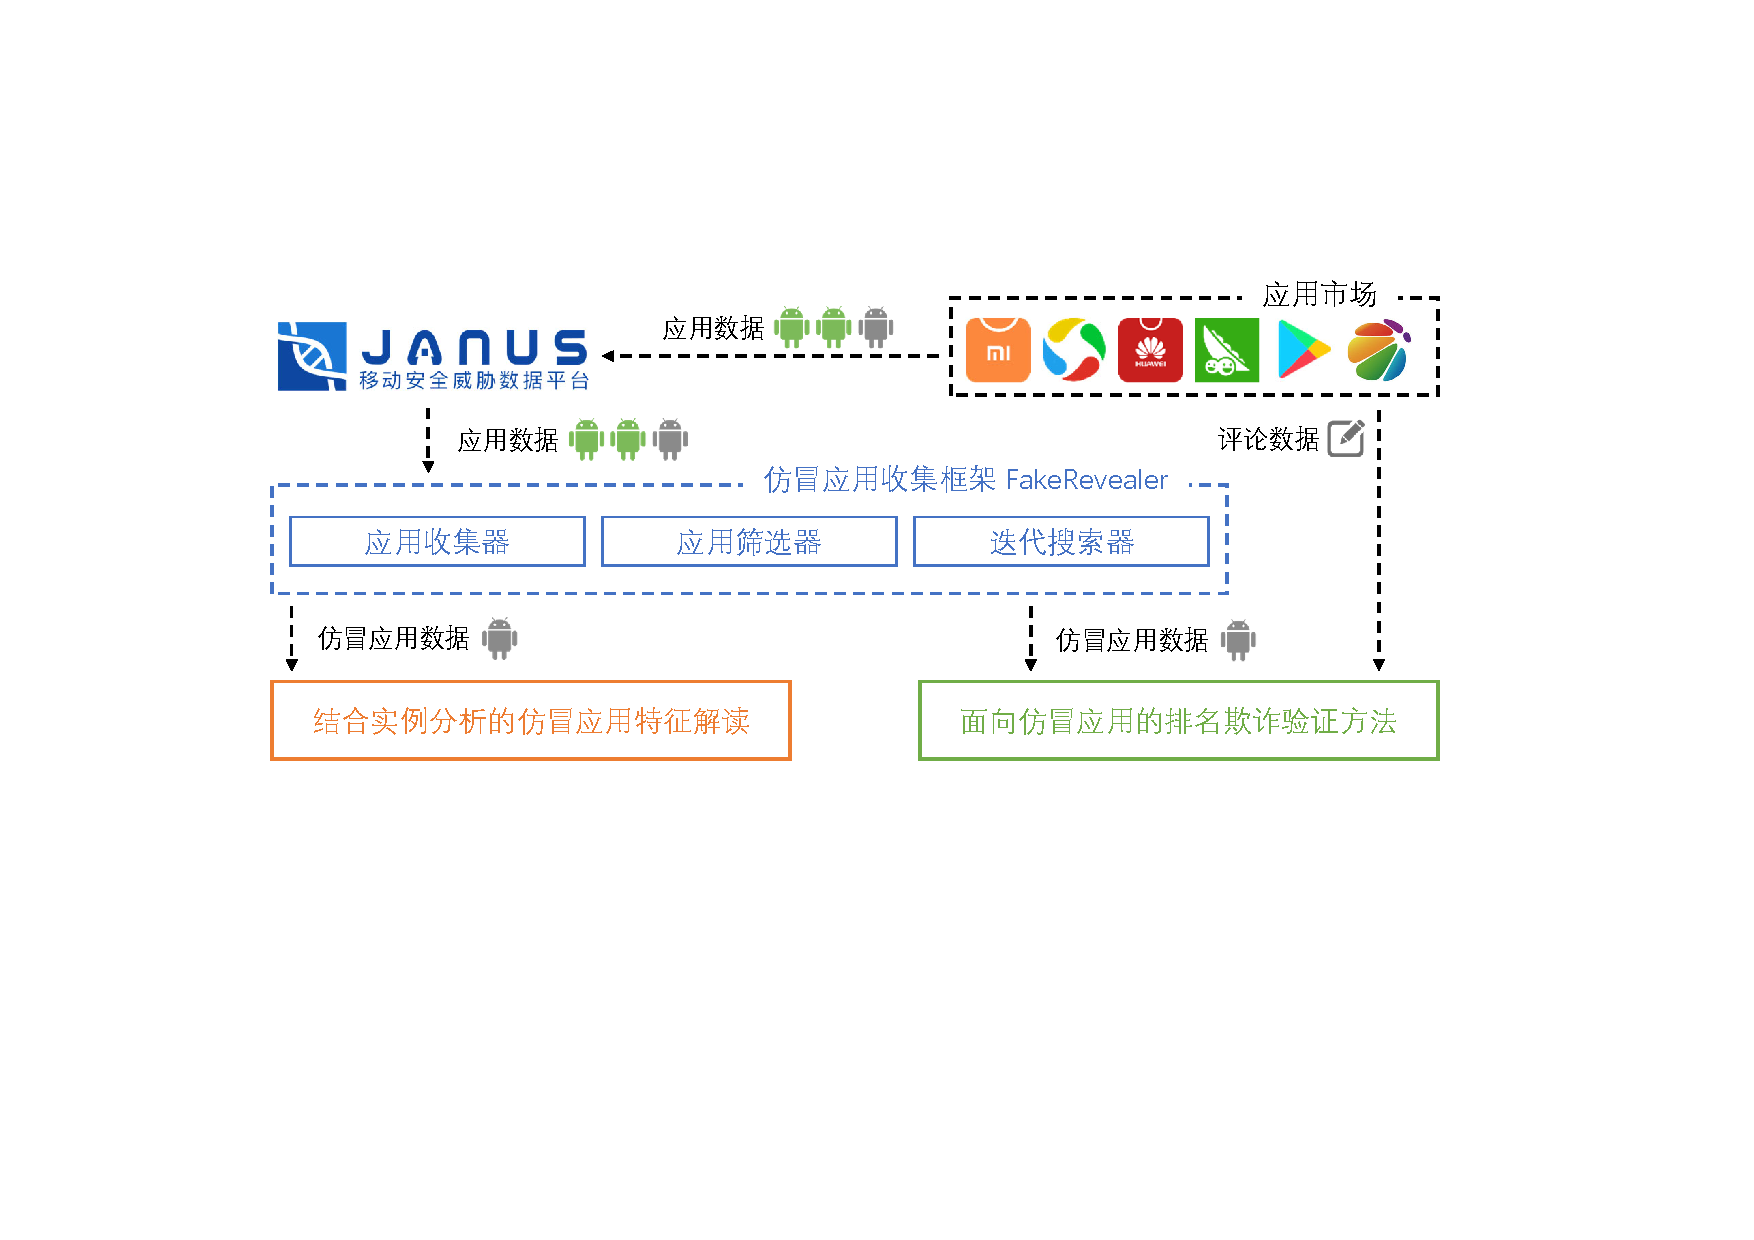
\includegraphics[width=\textwidth]{./Figures/edwin-overview}
	\caption{本文研究流程}
	\label{fig:Workflow}
	\vspace{-3mm}
\end{figure}

% Fig.~\ref{fig:Workflow} shows the workflow of our study, which can be divided into two main phases:
\autoref{fig:Workflow} 展示了本次实证研究的流程,其可以分为四个主要阶段:

1)\ \emph{数据收集} \quad
数据收集主要分为两个部分:正版应用信息的收集和仿冒应用的收集。
在正版应用信息收集的部分,本文选择了50个最热门的App作为目标App,然后手动收集了跟这些App有关的信息;
仿冒应用信息收集方面,作者得到了上海犇众信息技术有限公司的帮助,得以接触从各个应用商店获得的大量的应用样本。
借助自动化分析框架\mytool,作者获得了大量仿冒应用的数据。

2)\ \emph{大规模数据挖掘} \quad
在这一步,我们对搜集到的仿冒样本数据进行分析,从三个视角完成了一次大规模数据挖掘。
三个视角分别是仿冒的基本应用特征、影响仿冒应用数量的因素和仿冒应用的发展轨迹,由浅入深,帮助读者理解仿冒应用的生态。

3)\ \emph{仿冒案例分析} \quad
之后,我们从收集的数据中选择了3个案例进行更深入的分析。
这三个案例在支持数据挖掘中的发现之外,揭示了更多仿冒应用开发者的行为特征。

4)\ \emph{市场反馈分析} \quad
在这个部分,我们从第三方应用市场中随机选取一部分应用,提取了用户对它们的所有历史评价,然后筛选出其中对仿冒应用的评价并分析,以期了解用户对这些应用持有的态度。
此基础上,我们还检测了仿冒应用与排名欺诈行为的关系,揭示移动黑灰产不同环节之间的关联。

\section{应用数据收集}
鉴于目前学术界中未有相关工作能提供仿冒应用的相关数据集,本研究率先尝试着从工业界中系统地收集所需的仿冒应用数据。
然而仿冒应用是一个跟正版应用相对的概念,所以本文需要先定义正版应用,再根据正版应用的信息搜寻仿冒应用。

\subsection{收集流程简介}
1)\ \emph{正版应用收集} \quad
在定义正版应用方面,本研究参考了数据平台易观千帆的月度App排行榜\footnote{\url{https://qianfan.analysys.cn/refine/view/rankApp/rankApp.html}},然后从中选出了其中的前50款热门App作为本次研究的目标App。
之后,作者手动地从这50款App的官方网站上下载了这些应用的最新版本,作为正版应用的参考版本。

2)\ \emph{仿冒应用收集} \quad
要获取足量的仿冒应用数据以组成数据集是一个十分具有挑战性的任务,难点如下:
\begin{itemize}
	\item 研究者要从多个不同的应用市场中爬取App样本,每个应用市场都有不同的网页编码,不存在一个爬虫脚本对所有应用市场数据都通用的场景;
	\item 各个应用市场架上的App数量浩如繁星,研究者需要有效地找到和目标App有关的所有样本,不重不漏;
	\item 对于大量数据,研究者需要一个轻量级的解决方案快速判断获得的App样本究竟为正版应用又或者是仿冒应用。
\end{itemize}

为了应对第一个挑战,作者与工业界合作,利用犇众信息公司的Janus平台对各大应用商店进行样本爬取,从而获得大量应用样本。
事实上,如\autoref{fig:Janus-data}显示,Janus平台自2017年起就开始对各大应用商店的App进行样本收集,至今已收集到上千万个App样本。
除样本搜集外,Janus也提供按规则搜索功能,用户可以创建自己的规则过滤平台中的应用数据,以获取自己需要的App样本。

\begin{figure}[htbp]
	\centering
	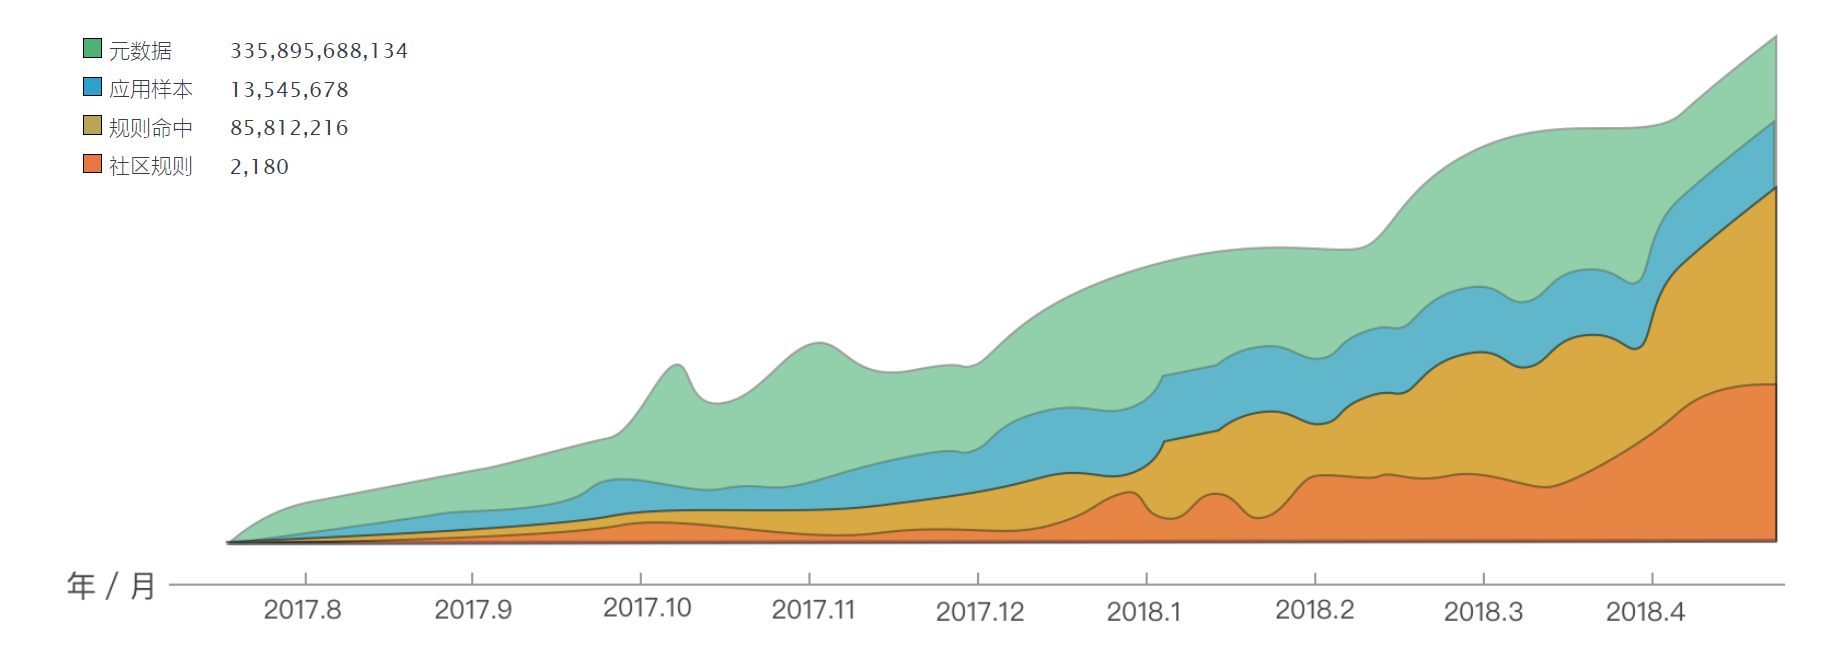
\includegraphics[width=\textwidth]{./Figures/edwin-Janus-data.png}
	\caption{Janus平台上的数据规模时序图}
	\label{fig:Janus-data}
	\vspace{-5mm}
\end{figure}

为了应对第二个和第三个挑战,作者搭建了应用筛选框架\mytool。
利用一个基于广度优先搜索(Breadth-First Search,简称BFS)的算法,作者在\mytool 中实现了一个\componentB ,以应用的\emph{包名}和\emph{应用名}作为拓展数据项,从Janus平台中分步迭代搜索与目标应用相关的所有App样本,然后将相关样本下载到本地保存;
对下载到本地的应用,作者使用\mytool 的组件\componentA 提取所需的数据;
然后,基于前述收集到的正版应用信息,作者在\mytool 中构建出了一个\componentC ,将上一步中提取到的数据和正版应用作比对。

关于应用数据收集流程的详细信息,可以参考\fullref{chp:fakerevealer}的介绍。

% \noindent {\bf Collected Dataset.}
\subsection{应用数据概览}
以下是框架收集到的数据的概览:

从易观千帆提供的数据榜单中,本研究选择了50个最热门的App作为目标App,这些App分属11个不同的应用类别。
由于App的应用名可能会在App更新迭代的时候随之变更,作者用近似BFS的策略,从50种App中一共记录了198个不同的应用名,来挖掘仿冒样本。

在这50款App中,以下三款App的样本并不能在市面上找到:\emph{OPPO 应用商店},\emph{华为应用商店}和\emph{小米应用商店}。
因为这三款App都是由手机设备厂商开发和预装在对应品牌的手机中的,仅供这些品牌的用户使用,并不在其他应用市场上提供下载。
当然,这也是这三款App热度高的原因——这几款App都被预装到了对应手机品牌厂商的每一部Android设备中,而OPPO、华为和小米又是国内最大的几家手机厂商,这几款App自然也会有庞大的用户基数。
因此,本研究最后的目标App只有47款。

对这47款目标App,作者总共收集到了138,106个应用样本。
其中,69,614个应用样本持有官方开发者证书,52,638个应用样本并不具有官方证书。
还有一部分应用样本,是某些应用的分别发布在不同应用市场同一版本,在经过去重筛选后被排除(共计15,854个)。

对于每个样本,框架会收集8个数据项作为元数据:\emph{样本SHA1码},\emph{安全证书SHA1码},\emph{包名},\emph{样本大小},\emph{版本号},\emph{搜集时间}和\emph{APK包来源}。
其中,\emph{样本SHA1码}是使用SHA1哈希算法对整个APK文件进行数据摘要之后获取到的编码串,每个样本都有独一无二的SHA1码;安全证书SHA1码则是对样本的安全证书采用SHA1算法提取数据摘要之后获取的编码串,用于识别不同的证书。
而\emph{搜集时间}则是样本从应用市场被爬取到数据库的时间点,\emph{APK包来源}指示该APK包来源的应用市场。

\section{本章小结}

本章主要对本研究进行了概览,介绍了数据收集的流程和方法,然后对采集到的数据进行了简要描绘。
% Empirical study is then applied to these metadata, especially to those of fake apps, to gain us a more comprehensive understanding on fake apps' nature and characteristics, and the behaviors of fake app authors.
下一章,我们将详述数据收集工具\mytool 的设计和实现。
